%\documentclass[aps,prl,showpacs,superscriptaddress,amsmath,amssymb,obeyspaces]{revtex4}

\documentclass{article}
\usepackage{hyperref}
\usepackage{graphicx}% Include figure files
\usepackage{listings}
\usepackage{tikz}
\usetikzlibrary{trees}
\usepackage{amsmath}
\usepackage{amssymb}
\usepackage{color}
\usepackage{booktabs}
\definecolor{mygreen}{rgb}{0,0.6,0}
\definecolor{mygray}{rgb}{0.5,0.5,0.5}
\definecolor{mymauve}{rgb}{0.58,0,0.82}


 \definecolor{darkgreen}{rgb}{0.3,0.5,0.3}
 \definecolor{darkblue}{rgb}{0.3,0.3,0.5}
 \definecolor{darkred}{rgb}{0.5,0.3,0.3}
 \lstdefinelanguage{LUA}{%
  sensitive=true,%
  columns=fixed,%
  keywordstyle=[1]{\color{darkblue}\bfseries},%
  keywordstyle=[2]{\color{darkgreen}\bfseries},%
  morekeywords=[1]{local,if,then,else,end,while,do, coroutine,yield},% Official LUA keywords
  morekeywords=[2]{SMA_Handle, Controller, handle, Output, FindFile},% Your private keywords
  otherkeywords={.,=,~,*,>,:},%
  morestring=[b]",%
  stringstyle={\color{darkred}\itshape},%
  breaklines=true,%
  linewidth=\textwidth,%
  comment=[l]{--}%
 }



\lstset{ %
  backgroundcolor=\color{white},   % choose the background color; you must add \usepackage{color} or \usepackage{xcolor}
  basicstyle=\footnotesize,        % the size of the fonts that are used for the code
  breakatwhitespace=false,         % sets if automatic breaks should only happen at whitespace
  breaklines=true,                 % sets automatic line breaking
  captionpos=b,                    % sets the caption-position to bottom
  commentstyle=\color{mygreen},    % comment style
  deletekeywords={...},            % if you want to delete keywords from the given language
  emph = {force, Force, Integrator},      % ProtoMol conf keyword
  emphstyle = {\bfseries}, % Keyword style
  escapeinside={\%*}{*)},          % if you want to add LaTeX within your code
  extendedchars=true,              % lets you use non-ASCII characters; for 8-bits encodings only, does not work with UTF-8 
 frame=single,                    % adds a frame around the code
  keepspaces=true,                 % keeps spaces in text, useful for keeping indentation of code (possibly needs columns=flexible)
  keywordstyle=\color{blue},       % keyword style
  language=bash,                 % the language of the code
  morekeywords={*,...},            % if you want to add more keywords to the set
  numbers=left,                    % where to put the line-numbers; possible values are (none, left, right)
  numbersep=5pt,                   % how far the line-numbers are from the code
  numberstyle=\tiny\color{mygray}, % the style that is used for the line-numbers
  rulecolor=\color{black},         % if not set, the frame-color may be changed on line-breaks within not-black text (e.g. comments (green here))
  showspaces=false,                % show spaces everywhere adding particular underscores; it overrides 'showstringspaces'
  showstringspaces=false,          % underline spaces within strings only
  showtabs=false,                  % show tabs within strings adding particular underscores
  stepnumber=10,                    % the step between two line-numbers. If it's 1, each line will be numbered
  stringstyle=\color{mymauve},     % string literal style
  tabsize=2,                       % sets default tabsize to 2 spaces
  title=\lstname                   % show the filename of files included with \lstinputlisting; also try caption instead of title
}
\usepackage{courier}

\lstset{basicstyle=\footnotesize\ttfamily,breaklines=true}
%\lstset{framextopmargin=50pt,frame=bottomline}

\begin{document}
\begin{section} {Introduction}
 According to its website, \textsc{ProtoMol} is an ``object-oriented, component based, framework for molecular dynamics (MD) simulations''. It was first developed in 2004 and its most recent version is v3.0. Written in \textsc{C++},  \textsc{ProtoMol} can simulate common classical mechanics with very high efficiency. Although it was designed originally for chemistry/biochemistry simulation, it has been succesfully adapted to simulate ion trap dynamics. For a detailed review of \textsc{ProtoMol}, please see Ref. 
\end{section}
{section} {Obtaining \textsc{ProtoMol}}
\textsc{ProtoMol} is open-source and cross platform. The source code of \textsc{ProtoMol} is hosted at \textsc{sourceforge}, and the download URL is \url{http://sourceforge.net/projects/protomol/files/ProtoMol/Protomol 3.3/} for each platform. The Linux version used in Hudson lab simulations has undergone considerable modification, so I highly recommend downloading the modified version to start with. The address is \url{https://github.com/kuangchen/ProtoMol}. Any \textsc{git} tool should be able to clone this online repository into local copies.

\end{section}
\begin{section} {Compiling \textsc{ProtoMol}}
The compilation of original \textsc{ProtoMol} source code do not require any additional external programming libraries. The modified version however, requires the following libraries, to be installed first. 
\begin{itemize}{}{}
\item Lua5.2
\item HDF5
\end{itemize}
On Ubuntu/Linux systems, these packages can be installed by \textsc{apt-tools}. On Windows, these packages can be found at \url{http://code.google.com/p/luaforwindows/}, and \url{http://www.hdfgroup.org/HDF5/release/obtain5.html}. As for the compiler, because some new features introduced in C++11 are used, a compatible C++ compiler should be used. The compilation process have been simplified by \textsc{CMake} tool. On Linux machine, installation is accomplished by the following commands, 
\lstset{language=bash} 
\begin{lstlisting}
# Remove previous CMakeCache
rm -rf CMakeCache.txt CMakeFiles

# Instructs ProtoMol to have lapack built
cmake -DBUILD_LAPACK=ON -DBUILD_LAPACK_TYPE=lapack 

# Tell cmake to generate Makefiles
cmake .

# Install ProtoMol into system folder, as super user
sudo make install
\end{lstlisting}
\end{section}

\begin{section} {Basic Usage}
Either through GUI interface or console, a user defines a simulation configuration file that instructs \textsc{ProtoMol} about simulation initial conditions, integrator, outputs, and other properties of simulation. The configuration file consists of entries in the format of ``keyword value'' pair. The most important part of the configuration file is the declaration of integrators and forces, which have their special syntax. 

An example input file is presented below, with the meaning of each keyword given in the comment line. To see a full list of keywords, please refer to Ref.
\begin{lstlisting}[frame=single]
# Number of steps in simulation
numsteps 100000000
firststep 0

# Random Number seed
seed 11
temperature 1e4

# Simulation cell size
cellsize 5000000

# Boundary Conditions
boundaryConditions vacuum

# Cell Manager
cellManager Cubic
exclude none

# Initial position and velocitiy definition
posfile ion_neutral_cooling_ini_pos_32.xyz
psffile ion_neutral_cooling_32.psf

# Par file definition
parfile ion_neutral_cooling.par

# Output Setting
outputfreq 10000
IonSnapshot ss.lua

# Integrator Setting
Integrator {
  # 0th level integrator
  level 0 LeapfrogBufferGas {
    timestep 1e8
    filename buffer_gas.lua	
        
    # Add Coulomb force between ions
    force Coulomb 
    -algorithm NonbondedSimpleFull
        
    # Add Linear Quadrupole Trap force
    force LQT 
    -lqt_filename trap.lua
  }
}
\end{lstlisting}
\end{section}

\begin{section} {Using the ProtoMol Addons}
Although \textsc{ProtoMol} is a powerful MD simulation software, it does not meet every specific simulation goals right out of box. Modification and extension of the source codes are needed, to achieve these goals. In this section, I will present the usage of the extensions I wrote in particular for the ion trap simulation.

\begin{subsection} {Force from the trapping field}
To define the force from the trapping rf-field, the following force specification should be added to the integrator. 
\begin{lstlisting}[language=bash]
force LQT 
-lqt_filename trap.lua
\end{lstlisting}
filename specifies the filename of trap definition, which is written in the language of Lua. An example file of trapp definition file is given below,
\begin{lstlisting}[language=LUA]{Example trap definition file}
trap = { m = 173, -- AMU
  r0 = 12e-3,     -- m
  z0 = 21.5e-3,   -- m
  v_rf = 175/2,   -- V
  v_ec = 10,      -- V
  eta = 0.1275,   -- 1
  omega = 300e3   -- Hz
}
\end{lstlisting}
The trap definition declares a variable trap, a Lua table that defines an ion trap through its fields. The meaning of each field is given by Eq. \footnote{The ion is assumed to be singly charged. For multiply-charged ion, ion's mass needs to be scaled accordingly.}. The unit of each quantity is given in the comment. 
\end{subsection}

\begin{subsection} {Harmonic trap force}
If one is not concerned about rf-heating, one can use the pondermotive potential to approximate the real trap potential. 
\begin{lstlisting}[language=bash]
force HarmonicTrapForce
-ht_def ht_trap.lua
\end{lstlisting}
where -ht\_def points to a lua file that defines the trapping frequency.
\begin{lstlisting}[language=LUA]{Example trap definition file}
trap = { freq = { x = 39.63e3 * 2 * 3.14159,
                  y = 39.63e3 * 2 * 3.14159,
                  z = 39.63e3 * 2 * 3.14159 } }
\end{lstlisting}
The trap definition declares a variable trap, a Lua table that contains a single field freq, which in turn contains three field x, y, z. The meanings and units of these field are given in the following table.
\begin{table}[h!]
  \centering
  \begin{tabular}{ c  c  l } \toprule
    Field & Unit & Meaning\\ \midrule
    $\omega_x$ & Hz & trapping frequency defined by $V=\frac{1}{2}(\omega_x^2x^2+\omega_y^2y^2+\omega_z^2z^2)$\\
    $\omega_y$ & Hz &   \\
    $\omega_z$ & Hz &   \\ \bottomrule
  \end{tabular}
  \caption{Damping Force Definition File}
  \label{tab:harmonic_trap_def}
\end{table}


\end{subsection}
\begin{subsection} {Damping force}
The damping force is introduced to emulate the laser-cooling force, which quickly removes ions' kinetic energy, and cause the ions to form Coulomb crystal. The damping force is added to the simulation by
\begin{lstlisting}
force DampingForce
-damping_def damping.lua
\end{lstlisting}
where -damping\_def points to a lua file that defines the damping coefficient, and the duration when the damping is on.
\begin{lstlisting}[language=LUA]{Example trap definition file}
  damping = { coeff = 3e-22,
    t_start = -1,
    t_end = 0.01 }
\end{lstlisting}


\begin{table}[h!]
  \centering
  \begin{tabular}{ c  c  l } \toprule
    Field & Unit & Meaning\\ \midrule
    coeff & ? & damping coeffient $b$, defined by $\mathbf{F}=-b\mathbf{v}$\\
    t\_start & sec & start time  \\
    t\_end & sec & end time  \\ \bottomrule
  \end{tabular}
  \caption{Damping Force Definition File}
  \label{tab:damping_def}
\end{table}

\end{subsection}

\begin{subsection} {Leap Frog Buffer Gas Integrator V2}
To introduce collisions with ultracold neutral atoms, a leap frog integrator is written. An example input is given by
\begin{lstlisting}
level X LeapFrogBufferGas2 {
  timestep 1e8
  filename buffer_gas.lua
}
\end{lstlisting}
where buffer\_gas\_def points to the buffer gas definition file.
\begin{lstlisting}[language=LUA]{Example trap buffer_gas file}
  neutral = { mass = 40,
    polarizability = 50,
    temperature = 5e-3,
    density = 1e16 }

  trap = { radius = 12e-3, 
    z0 = 21.5e-3 }
\end{lstlisting}


\begin{table}[h!]
  \centering
  \begin{tabular}{ c  c  l } \toprule
    Field & Unit & Meaning\\ \midrule
    mass & AMU & mass of neutral atom \\
    polarizability & $10^{24} cm^3$ & polarizability of neutral atom \\
    temperature & Kelvin & temperature of neutral atom \\
    density & $m^3$ & density of neutral atom
  \end{tabular}
  \caption{Buffer Gas Definition Part I}
  \label{tab:leapfrogintegrator_def_p1}
\end{table}

\begin{table}[h!]
  \centering
  \begin{tabular}{ c  c  l } \toprule
    Field & Unit & Meaning\\ \midrule
    radius & $m$ & radius of ion trap \\
    polarizability & $10^{24} cm^3$ & polarizability of neutral atom \\
    temperature & Kelvin & temperature of neutral atom \\
    density & $m^3$ & density of neutral atom
  \end{tabular}
  \caption{Buffer Gas Definition Part II}
  \label{tab:leapfrogintegrator_def_p2}
\end{table}
\end{subsection}

\end{section}
\begin{subsection} {Ion Snapshot}
  \begin{subsubsection} { Terminology: Snapshot and Frame }
    A user might want to record each ion's position and velocity at various times in the simulation. Let's call these information \emph{snapshots}. Unlike what it litarally sounds, a snapshot couldeither include ion's instaneous positions and velocities information at a single time step, called \emph{frame}, or a consecutive series of frames.
    For my implementation of ion snapshots, every snapshot contains same number of frames. So to specify how ion snapshots should be stored, a user need to provide the start time $t_i$ for $i^{th}$ snapshot with $i=0, 1, ... N_s$ and number of frames $N_{f}$ in each snapshot.
  \end{subsubsection}


  \begin{subsubsection} {Syntax}
    The statement to instruct \textsc{ProtoMol} to write snapshots to files on disk is
    \begin{lstlisting}[emph=IonSnapshot]
      IonSnapshot filename\end{lstlisting}
    where \textbf{IonSnapshot} points to a lua file that defines these snapshots. An example snapshot definition file is presented below,
    \begin{lstlisting}[language=LUA]{Example file of snapshot definition}
      start_time = {}

      for i=1, 50 do
        start_time[i] = (i-1) * 2e-2
      end

      ss = {
        num_frame = 250, 
        start = start_time 
      }

      dir = ./\end{lstlisting}
    which should always declare a table variable \emph{ss}, with the fields explained in Tab. 
    \begin{table}[h!]
      \centering
      \begin{tabular}{l  l  l  p{7cm} } \toprule
        Field & Type &  Unit & Meaning\\ \midrule
        num\_frame & integer & 1 & $N_f$, if set to -1, then $N_f$ set to number of steps  in the longest secular periods in $x,y,z$ three directions \\ 
        start & table & sec & $t_i$, i.e. the time of the first frame \\
        dir & string & N/A & The name of directory where snapshot files are stored\\
        \bottomrule
      \end{tabular}
      \caption{Snapshot Definition}
      \label{tab:ion_snapshot_def}
    \end{table}
  \end{subsubsection}

\begin{subsubsection} {Output Directory Structure}
All the snapshot files are stored under the same directory, specified by the \textbf{dir} keywords in the definition file. They are named by the pattern snapshot\_$i$.hd5, where $i$ ranges from $0$ to $N_s-1$.
\tikzstyle{every node}=[draw=black,thick,anchor=west]
\tikzstyle{selected}=[draw=red,fill=red!30]
\tikzstyle{optional}=[dashed,fill=gray!50]
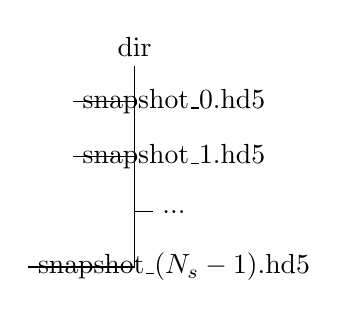
\begin{tikzpicture}[%
  grow via three points={one child at (0.5,-0.7) and
  two children at (0.5,-0.7) and (0.5,-1.4)},
  edge from parent path={(\tikzparentnode.south) |- (\tikzchildnode.west)}]
  \node {dir}
    child { node {snapshot\_$0$.hd5} }
    child { node {snapshot\_$1$.hd5} }
    child { node {...} }
    child { node {snapshot\_$(N_s-1)$.hd5} };
\end{tikzpicture}
\end{subsubsection}


\begin{subsubsection} {Snapshot File Structure}
The snapshot files are stored in HDF5 format, for its compact size and support by major programming languages, including C/C++/Python/Matlab. For an overview of HDF5 file, please visit its official website at \url{http://www.hdfgroup.org/HDF5/}.

Every HDF5 file has a hierachical data structure, very similar to the file system structures in an operating system. In addition to $N_f$ consecutive frames, a \textit{config} header is also included which consists of auxillary information intended to make the snapshot file self-inclusive.
\tikzstyle{every node}=[draw=black,thick,anchor=west]
\tikzstyle{selected}=[draw=red,fill=red!30]
\tikzstyle{optional}=[dashed,fill=gray!50]
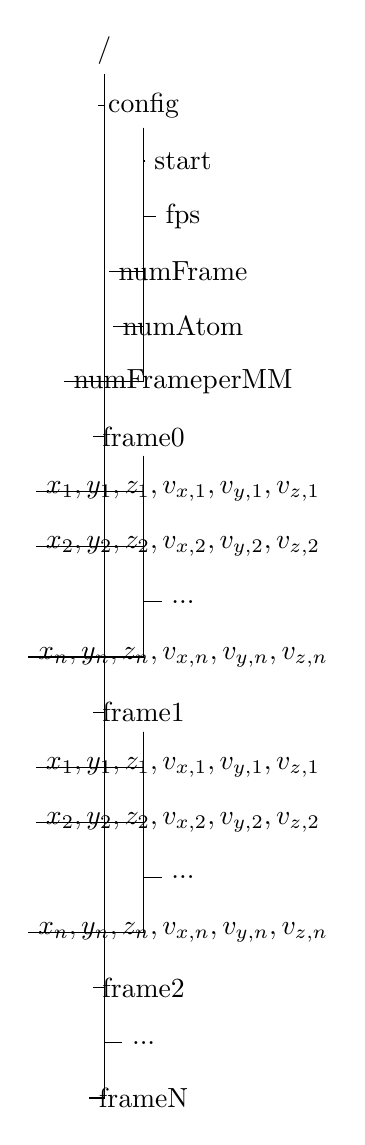
\begin{tikzpicture}[%
  grow via three points={one child at (0.5,-0.7) and
  two children at (0.5,-0.7) and (0.5,-1.4)},
  edge from parent path={(\tikzparentnode.south) |- (\tikzchildnode.west)}]
  \node {/}
    child { node {config} 
      child { node {start} }
      child { node {fps} }
      child { node {numFrame} }
      child { node {numAtom} }
      child { node {numFrameperMM} }
    }
    child [missing] {}				
    child [missing] {}				
    child [missing] {}				
    child [missing] {}				
    child [missing] {}	
    child { node {frame0} 
      child {node {$x_1, y_1, z_1, v_{x,1}, v_{y,1}, v_{z,1}$} } 
      child {node {$x_2, y_2, z_2, v_{x,2}, v_{y,2}, v_{z,2}$} } 
      child {node {...} } 
      child {node {$x_n, y_n, z_n, v_{x,n}, v_{y,n}, v_{z,n}$} }
    }
    child [missing] {}				
    child [missing] {}				
    child [missing] {}				
    child [missing] {}			
    child { node {frame1} 
      child {node {$x_1, y_1, z_1, v_{x,1}, v_{y,1}, v_{z,1}$} } 
      child {node {$x_2, y_2, z_2, v_{x,2}, v_{y,2}, v_{z,2}$} } 
      child {node {...} } 
      child {node {$x_n, y_n, z_n, v_{x,n}, v_{y,n}, v_{z,n}$} }
    }
    child [missing] {}				
    child [missing] {}				
    child [missing] {}				
    child [missing] {}			
    child { node {frame2} }
    child { node {...} }
    child { node {frameN} };
\end{tikzpicture}
\end{subsubsection}
\end{subsection}

\begin{section} {Writing your own \textsc{ProtoMol} extensions}
\begin{subsection} {Adding a new force}
  
\end{subsection}

\begin{subsection} {Adding a new integrator}
  
\end{subsection}

\begin{subsection} {Adding a new output}
  
\end{subsection}



\end{section}
\end{document}
 
%  LocalWords:  overline
